\algblockdefx{RepeatUntil}{EndRepeatUntil}{\textbf{repeat until}}{}
\algnotext{EndRepeatUntil}

\section{Semi-Analytical Primal Solver}
\label{sec:sap_solver}

Our Semi-Analytical Primal Solver, or SAP for short, essentially is a Newton
iteration used to find the minimum of the unconstrained formulation stated in
Eq. (\ref{eq:primal_unconstrained}), where constraints have been eliminated
using our analytical inverse dynamics. At each $m\text{-th}$ Newton iteration,
SAP uses analytical expressions of both the gradient and Hessian of
$\ell_p(\mf{v})$, with line search to find the unique optimal solution
\begin{algorithm}[H]
	\caption{SAP Newton Iteration}	
	\begin{algorithmic}
	\State Initialize $\mf{v}^0 \gets \mf{v}_0$
	\RepeatUntil $~\Vert\tilde{\nabla}\ell_p\Vert < \varepsilon_a + \varepsilon_r\max(\Vert\tilde{\mf{p}}\Vert,\Vert\tilde{\mf{j}_c}\Vert)$, Eq. \eqref{eq:stopping_criteria}
	\State $\displaystyle \Delta\mf{v}^{m} = -\mf{H}^{-1}(\mf{v}^m)\nabla_\mf{v}\ell_p(\mf{v}^m)\nonumber$
	\State $\displaystyle \alpha^m = \argmin_{t\in\mathbb{R}^{++}} \ell_p(\mf{v}^m + t \Delta\mf{v}^{m})$
	\State $\displaystyle \mf{v}^{m+1} = \vf{v}^m + \alpha^{m}\Delta\mf{v}^{m}$
	\EndRepeatUntil
	\State\Return $\mf{v}$, $\bgamma=P_\mathcal{F}(\vf{y}(\mf{v}))$
\end{algorithmic}
\end{algorithm}
where we use the previous time step velocity $\mf{v}_0$ to initialize the
iteration. The stopping criteria is discussed in below in Section
\ref{sec:stopping_criteria}.

Specifics of the line search algorithm are critical to the success of the SAP
solver given that the cost can undergo large changes as $\mf{v}^m$ explores
states corresponding to different contact modes. We explored two line-search
algorithms: an approximate backtracking line-search with Armijo's stopping
criteria and an exact (to machine epsilon) line-search. We show how a careful
pre-computation of commonly occurring terms enables the exact line-search step
for a small fraction of the total cost. While backtracking line-search with
Armijo's rule guarantees the convergence of SAP, we found out that exact
line-search can lead to a performance improvement between 15\% to 35\%. In the
next subsections we describe each component of the solver in detail.

\subsection{Gradients}
\label{sec:gradients}

%Appendix \ref{app:gradients_derivation}

We summarize the main results required for implementation. The gradient of the
primal cost $\ell_p$ is
\begin{equation}
	\nabla_\mf{v}\ell_p(\mf{v}) = \mf{A}(\mf{v}-\mf{v}^*) + \nabla_\mf{v}\ell_R,
\end{equation}
where we defined the regularizer cost as $\ell_R(\mf{v})=\frac{1}{2}\Vert
P_\mathcal{F}(\mf{y}(\mf{v}))\Vert_R^2$. We show in Appendix
\ref{app:gradients_derivation} that this gradient can be computed analytically,
with the result
\begin{equation}
	\nabla_\mf{v}\ell_p(\mf{v}) = \mf{A}(\mf{v}-\mf{v}^*) - \mf{J}^T\bgamma(\mf{v})
	\label{eq:primal_gradient}
\end{equation}
with $\bgamma(\mf{v})=P_\mathcal{F}(\vf{y})$ from the analytical inverse
dynamics in Eq. \eqref{eq:analytical_y_projection}. This recovers the original
momentum balance in Eq. (\ref{eq:momentum_linearized}) since Newton's method
solves for $\nabla_\mf{v}\ell_p=\mf{0}$.

We obtain the Hessian $\mf{H}=\nabla_\mf{v}^2\ell_R$ by taking the gradient of
Eq. (\ref{eq:primal_gradient}). The result is
\begin{eqnarray}
	\nabla_\mf{v}^2\ell_R(\mf{v}) &=& \mf{J}^T\mf{G}\,\mf{J}\nonumber\\
	\mf{G} &=&-\nabla_{\mf{v}_c}\bgamma = \nabla_\mf{y}\bgamma \mf{R}^{-1}
	\label{eq:ellR_hessian}
\end{eqnarray}
where $\nabla_{\mf{v}_c}\!\bgamma$ is a block diagonal matrix where each
diagonal elements is the $3\times 3$ matrix $\nabla_{\mf{v}_{c,i}}\!\bgamma_i$
for the $i\text{-th}$ contact. As shown in Appendix
\ref{app:gradients_derivation}, $\nabla_{\mf{v}_c}\bgamma\succeq 0$ and thus
$\nabla_\mf{v}^2\ell_R(\mf{v})\succeq 0$.

Finally, the Hessian needed in Newtons's method is
\begin{equation}
	\mf{H}= \mf{A} + \mf{J}^T\mf{G}\,\mf{J}
	\label{eq:ell_hessian}
\end{equation}
which, since $\mf{A}\succ 0$, $\mf{H}$ is strictly positive definite. Notice
that to compute the requried gradient and Hessian we need analytical expressions
for the projection $P_\mathcal{F}(\vf{y})$ and its gradient
$\nabla_\mf{y}P_\mathcal{F}(\vf{y})$, both provided in Appendices
\ref{app:analytical_inverse_dynamics_derivations} and
\ref{app:gradients_derivation} respectively.

\subsection{Line Search}
At each $m\text{-th}$ Newton iteration, our implementation of the backtracking
line-search tests candidate steps lengths until Armijo's criteria \cite[\S
3.1]{bib:nocedal2006numerical} is satisfied
\begin{algorithm}[H]
	\caption{Backtracking line-search}	
	\begin{algorithmic}
	\State With $\rho \in (0, 1)$, $c \in (0, 1)$ and $\alpha_\text{Max}>0$
	\State $\alpha\gets \alpha_\text{Max}$ 
	\RepeatUntil $~\ell_p(\alpha) <
	\ell_p(\mf{v}^m) + c\,\alpha \frac{d\ell_p}{d\alpha}(\mf{v}^m)$ \State
	$\alpha\gets \rho\alpha$
	\EndRepeatUntil
	\State\Return $\alpha$
\end{algorithmic}
\end{algorithm}	
and we typically use $\rho=0.8$, $c=10^{-4}$ and $\alpha_\text{Max}=1.5$.

For our exact line-search, we make the following observations
\begin{enumerate}
	\item $\ell_p(\alpha)$ is strictly convex, i.e. there is a unique minimum.
	\item Newton steps are well formed since $d^2\ell_p/d\alpha^2>0$.
	\item $\ell_p(\alpha)$ is a piecewise $C^1$ function. In other words,
	$d\ell_p/d\alpha$ is continuous but $d^2\ell_p/d\alpha^2$ might not be.	
	\item Given the regularization used to model friction and stiff compliance,
	gradients of $\ell_p(\alpha)$ can undergo large changes, even within a
	region where $\ell_p(\alpha)$ is continuous.
\end{enumerate}

This led us to choose a one-dimensional strategy that is robust under these
conditions. We found the method \verb;rtsafe; in \cite[\S
9.4]{bib:numerical_recipes} to work the best. \verb;rtsafe; is one-dimensional
root finder that uses the Newton-Raphson method and switches to bisection
whenever Newton's method leads to an iterate outside a search bracket or
whenever its convergence is slow. Using analytical first and second derivatives,
our line search simply reduces to finding the unique root of $d\ell/d\alpha$
using the \verb;rtsafe; algorithm. We found this method to perform so well, that
we iterate $\alpha$ to a machine precision at a negligible impact on the
computational cost. In practice this is our preferred algorithm since it allow
us to use very tight regularization parameters without having to tune tolerances
in the line search. Moreover, we observed 15\%-35\% performance improvement when
compared to the backtracking line-search.

\subsection{Efficient Analytical Derivatives For Line Search}

\verb;rtsafe; requires the first and second derivatives of $\ell_p$, while the
backtracking method only requires the first derivative to verify Armijo's
stopping criteria. We show how to compute these gradients efficiently in
$\mathcal{O}(n)$ operations.

Defining $\ell(\alpha) = \ell_p(\mf{v}+\alpha\Delta\mf{v})$ we can compute first
and second derivatives with respect to $\alpha$ using the gradient and Hessian
\begin{eqnarray}
	\frac{d\ell}{d\alpha}&=&\Delta\mf{v}^T\nabla_\mf{v}\ell(\alpha)\nonumber\\
	\frac{d^2\ell}{d\alpha^2}&=&\Delta\mf{v}^T\nabla_\mf{v}^2\ell(\alpha)\Delta\mf{v}\nonumber
\end{eqnarray}

These are expensive to compute derivatives for general non-linear functions and
most line search variations in practice are approximations that avoid their
computation altogether. We show that first and second derivatives can be
computed efficiently given the structure of the problem.

Using the gradients from Section \ref{sec:gradients} we can write
\begin{eqnarray}
	\frac{d\ell_M}{d\alpha}(\alpha)&=&\Delta\mf{v}^T\mf{A}(\mf{v}(\alpha)-\mf{v}^*)\\
	\frac{d\ell_R}{d\alpha}(\alpha)&=&-\Delta\mf{v}^T\mf{J}^T\bgamma
\end{eqnarray}
and defining the change of constraint velocity
$\Delta\mf{v}_c=\mf{J}\Delta\mf{v}$ and change of momentum $\Delta\mf{p} =
\mf{A}\Delta\mf{v}$ we obtain the much simpler and faster to compute versions
\begin{eqnarray}
	\frac{d\ell_M}{d\alpha}(\alpha)&=&\Delta\mf{p}^T(\mf{v}(\alpha)-\mf{v}^*)\\
	\frac{d\ell_R}{d\alpha}(\alpha)&=&-\Delta\mf{v}_c^T\bgamma(\alpha)
\end{eqnarray}
which only require dot products that can be computed in $\mathcal{O}(n_v)$ and
$\mathcal{O}(n_c)$ respectively.

Using the same definitions we can write simple expressions for the second
derivatives as well
\begin{eqnarray}
	\frac{d^2\ell_M}{d\alpha^2}(\alpha)&=&\Delta\mf{v}^T\mf{A}\Delta\mf{v}=\Delta\mf{v}^T\Delta\mf{p}\\
	\frac{d^2\ell_R}{d\alpha^2}(\alpha)&=&-\Delta\mf{v}_c^T
	\nabla_{\mf{v}_c}\bgamma\Delta\mf{v}_c
\end{eqnarray}
where notice that $\frac{d^2\ell_M}{d\alpha^2}$ is independent of $\alpha$ and
can be precomputed before proceeding into the line search and
$\frac{d^2\ell_R}{d\alpha^2}$ only involves $\mathcal{O}(n_c)$ operations given
the structure of $\nabla_{\mf{v}_c}\bgamma$, a block diagonal matrix.

\subsection{Problem Sparsity}
\label{sec:problem_sparsity}

The Hessian in Eq. (\ref{eq:ell_hessian}) inherits a block sparse structure from
the specific contact configuration of the problem. We want to exploit this
structure when solving Eq. (\ref{eq:Newton_iteration}) at each Newton iteration.
To that end we use a supernodal Cholesky factorization  \cite[\S
9]{bib:davis2016survey}. Implementing this factorization requires construction
of a \emph{junction tree}.  For this we apply the algorithm
\cite{bib:smail2017junction}, using cliques of $\mf{J}\,\mf{J}^T$ as input. We
use the implementation from the Conex solver \cite{bib:permenter2020}.

The block sparsity of the Hessian is best described with an example. We organize
our multibody systems as a collection of articulated \emph{tree structures}, or
a \emph{forest}. Consider the system in Fig. (\ref{fig:sparsity_example}).
\begin{figure}[!h]
	\centering
	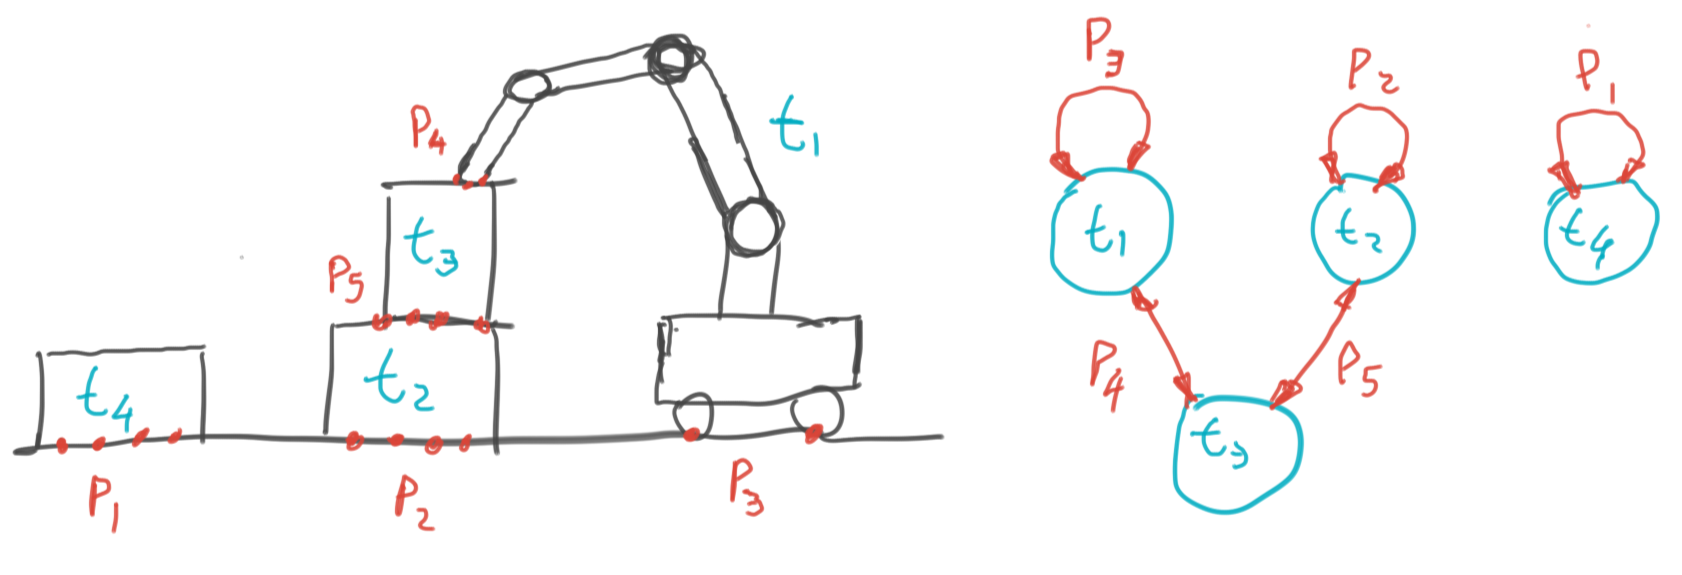
\includegraphics[width=0.7\columnwidth]{figures/sparsity_example.png}
	\caption{\label{fig:sparsity_example} 
	Example used to describe sparsity patterns commonly encountered in the
	simulation of robotic mechanical systems. The graph on the right puts
	\textit{trees} as nodes and contact \textit{patches} as edges. Notice how
	this graph exactly describes the sparsity pattern of the matrix
	$\mf{J}^T\mf{G}\mf{J}$ in Fig. \ref{fig:JTGJ_schematic}.}
\end{figure}
In this example a robot arm mounted on a mobile base constitutes its own tree,
here labeled $t_1$. The number of degrees of freedom of the $t\text{-th}$ tree
will be denoted with $n_t$. A free body is a special case of a tree where
$n_t=6$, this is a very common case. In general the mass matrix will have a
block diagonal structure where the $t\text{-th}$ diagonal block corresponds to
the mass matrix of the $t\text{-th}$ tree. For the example in Fig.
(\ref{fig:sparsity_example}) the mass matrix will look like\\\\
\begin{equation}
	\mf{M}=\quad
	\begin{bmatrix}
		\tikzmark{M_topleft}
		\diagentry{\mf{M}_{\cc{11}}}&&&\tikzmark{M_topright}\\
		&\diagentry{\mf{M}_{\cc{22}}}\\
		&&\diagentry{\mf{M}_{\cc{33}}}\\		
		\tikzmark{M_bottomleft}&&&\diagentry{\mf{M}_{\cc{44}}}
	\end{bmatrix}
% Draw lil arrows on top and to the left.
\tikz[overlay,remember picture] {
	\draw[->,thick,color=cyan]
  ([yshift=3ex]M_topleft) -- ([yshift=3ex]M_topright) node[midway,above]
  {\scriptsize $t$}; 
  \draw[->,thick,color=cyan]
  ([yshift=1.5ex,xshift=-2ex]M_topleft) -- ([xshift=-4ex]M_bottomleft)
  node[near end,left] {\scriptsize $t$};}	
\end{equation}
\RedHighlight{Make this equation a Figure instead.}

We define as \textit{patches} a collection of contact pairs between the same two
trees. We label in red all contact patches in Fig. (\ref{fig:sparsity_example}).
Each $i\text{-th}$ pair will correspond to a single cone constraint in our
formulation. The set of constraint indexes $i$ that belong to patch $p$ is
denoted with $\mathcal{I}_p$ of size (cardinality) $|\mathcal{I}_p| = r_p$.

Notice that our definition of \textit{patches} as used here to describe sparsity
has nothing to do with the actual geometrical topology of the contact surface
between two trees. That is, the \textit{patches} as defined here, could in
general correspond to a simple connected surface or even a complex contact area
formed by a set of disconnected surfaces. Figure (\ref{fig:sparsity_example})
labels trees and patches and shows the corresponding graph where the nodes are
the trees and the edges are the contact patches.

Recall from Eq. (\ref{eq:ellR_hessian}) that $\mf{G} =
-\nabla_{\mf{v}_c}\bgamma$ is a block diagonal matrix, with $\mf{G}_i =
\nabla_{\mf{v}_{c,i}}\bgamma_i \in \mathbb{R}^{3\times 3}$ at the $i\text{-th}$
diagonal block. We can write this also as $\mf{G} = \text{diag}(\mf{G}_p)$ if we
group contact pairs by patches to define $\mf{G}_p=\text{diag}(\mf{G}_i),
\,\forall i\in\mathcal{I}_p$.

The contact Jacobian will in general be sparse since the relative velocity at a
contact pair $i$ will only involve the generalized velocities of the two trees
in contact. For the case in Fig. (\ref{fig:sparsity_example}) the Jacobian will
look like\\\\
\begin{equation}
	\mf{J}=\quad
	\begin{bmatrix}
		\tikzmark{J_topleft}\mf{0} & 
		\mf{0} & \mf{0} & \mf{J}_{\rr{1}\cc{4}}\tikzmark{J_topright}\\		
		\mf{0} & \mf{J}_{\rr{2}\cc{2}} & \mf{0} & \mf{0}\\
		\mf{J}_{\rr{3}\cc{1}} & \mf{0} & \mf{0} & \mf{0}\\
		\mf{J}_{\rr{4}\cc{1}} & \mf{0} & \mf{J}_{\rr{4}\cc{3}} & \mf{0}\\
		\tikzmark{J_bottomleft}
		\mf{0} & \mf{J}_{\rr{5}\cc{2}} & \mf{J}_{\rr{5}\cc{3}} & \mf{0}		
	\end{bmatrix}
% Draw lil arrows on top and to the left.
\tikz[overlay,remember picture] {
	\draw[->,thick,color=cyan]
  ([yshift=3ex]J_topleft) -- ([yshift=3ex]J_topright) node[midway,above]
  {\scriptsize $t$}; 
  \draw[->,thick,color=red]
  ([yshift=1.5ex,xshift=-3ex]J_topleft) -- ([xshift=-3ex]J_bottomleft)
  node[near end,left] {\scriptsize $p$};}	
\end{equation}
\RedHighlight{Make this equation a Figure instead.}\\
where each non-zero block is the Jacobian $\mf{J}_{\rr{p}\cc{t}}$ of size
$3r_p\times n_t$.

We have now the elements to describe the sparsity of the product
$\mf{J}^T\mf{G}\mf{J}$. For the example in Fig. \ref{fig:sparsity_example}, the
block sparsity of $\mf{J}^T\mf{G}\mf{J}$ is illustrated in Fig.
\ref{fig:JTGJ_schematic}. Notice how the sparsity pattern of
$\mf{J}^T\mf{G}\mf{J}$ exactly matches the graph from Fig.
(\ref{fig:sparsity_example}). Finally the Hessian will have the sparsity
structure of $\mf{A} + \mf{J}^T\mf{G}\mf{J}$.
\begin{figure*}[!h]
	\centering
	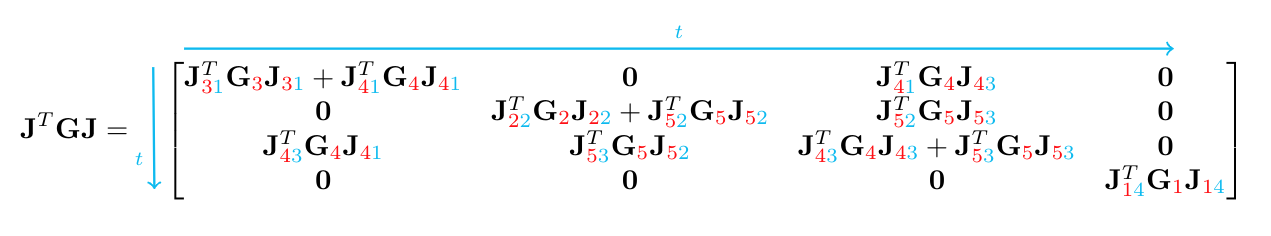
\includegraphics[width=0.8\textwidth]{figures/JTGJ_schematic.png}
	\caption{\label{fig:JTGJ_schematic} 
	Block sparsity of the $\mf{J}^T\mf{G}\mf{J}$ for the example illustrated in
	Fig. \ref{fig:sparsity_example}.}
\end{figure*}

Our implementation organizes the blocks of the Jacobian $\mf{J}$ as described in
this section, i.e. we condense rows by patches and columns by trees, so that the
supernodal Cholesky factorization can exploit this rich structure. Using this
block structure, the supernodal solver can take full advantage of specific
optimizations for dense algebra.



\subsection{Stopping Criteria}
\label{sec:stopping_criteria}

To assess convergence, we monitor the optimality condition for the unconstrained
problem in Eq. (\ref{eq:primal_unconstrained}) by evaluating the norm of the
momentum balance in Eq. (\ref{eq:primal_gradient})
\begin{equation}
	\nabla\ell_p(\mf{v}) = \mf{A}(\mf{v}-\mf{v}^*) - \mf{J}^T\bgamma.
\end{equation}

Notice that the components of $\nabla\ell_p$ have units of generalized momentum
$\mf{p}=\mf{M}\mf{v}$. Depending on the choice of generalized coordinates, the
generalized momentum components will have different units. In order to weigh all
components equally, we define the diagonal matrix $\mf{D} =
\text{diag}(\mf{M})^{-1/2}$ and perform the following change of variables
\begin{align}
	\tilde{\nabla}\ell_p &= \mf{D}\nabla\ell_p, \nonumber\\
	\tilde{\mf{p}} &= \mf{D}\mf{p}, \nonumber \\
	\tilde{\mf{j}}_c &= \mf{D}\mf{j}_c,
	\label{eq:scaled_momentum_quantities}
\end{align}
where we defined the generalized contact impulse $\mf{j}_c=\mf{J}^T\bgamma$.
With this scaling, all the new \emph{tilde} variables have the same units,
$\text{J}^{1/2}$. Using these definitions, we write our stopping criteria as
\begin{equation}
	\Vert\tilde{\nabla}\ell_p\Vert < \varepsilon_a + \varepsilon_r\max(\Vert\tilde{\mf{p}}\Vert,\Vert\tilde{\mf{j}_c}\Vert).
	\label{eq:stopping_criteria}
\end{equation}
where $\varepsilon_r$ is a dimensionless relative tolerance that we usually set
in the range $10^{-6}$ to $10^{-3}$. For all of our simulations in this paper,
we use $\varepsilon_r = 10^{-5}$. The absolute tolerance $\varepsilon_a$ is used
to detect rare cases where the solution leads to no contact and no motion,
typically due to externally applied forces. We always set this tolerance to a
small number, $\varepsilon_a=10^{-16}$.
